%% Quick build: [path]/convert.sh|pdflatex -synctex=1 -interaction=nonstopmode %.tex|biber %.bcf|pdflatex -synctex=1 -interaction=nonstopmode %.tex|pdflatex -synctex=1 -interaction=nonstopmode %.tex|evince %.pdf

\documentclass[doc]{apa6}
\usepackage[utf8]{inputenc}
\usepackage[english]{babel}
\usepackage{csquotes}
\usepackage[style=apa,sortcites=true,sorting=nyt,backend=biber]{biblatex}

\usepackage{amsmath}
\usepackage{amsfonts}
\usepackage{amssymb}
\usepackage{gensymb}
\usepackage[load=abbr]{siunitx}
\usepackage{setspace}	% for line spacing
\usepackage{calc}		% for figure scaling
\usepackage{svg}		% for graphics
\usepackage{graphicx}	% for graphics
\usepackage[left=1in,right=1in,top=1in,bottom=1in]{geometry}
\usepackage{listings}

%\DeclareLanguageMapping{american}{american-apa}
\addbibresource{/home/rob/Documents/bibtex/library.bib}

\linespread{1.5}

% Images are build by calling images/generate.sh <images> <output> where
% output is the "build" directory used by Texmaker.
\graphicspath{{./build/images/}}

\DeclareUnicodeCharacter{2010}{ }

%\lstset{%
%  basicstyle=\small\ttfamily,
%  language=Python
%}


\shorttitle{}

\title{Proposed Method for Using Cubic Splines for the Control of Remote-Sensing Unmanned Aerial Vehicles}
\author{Rob Skelly}
\affiliation{University of Victoria}
\note{Geography 590, Spring 2019}

%\abstract{}

\begin{document}

\maketitle



\section{Introduction}

In the field of remote sensing with unmanned aerial vehicles (UAVs), the maintenance of data quality is can be managed, in part, by stabilising the instrument-to-subject distance and orientation. This can be accomplished by controlling the vehicle's altitude and attitude, respectively.

UAV surveys are generally pre-planned using purpose-built software and followed (semi-)automonmously by the aircraft. Most currently-available software allows the creation of flight plans only in the horizontal plane \parencite[e.g.,][]{ArduPilot2018,DJI2018a,Microdrones2018,Group2018,UAVToolbox2018}, leaving it to the pilot to set a constant -- usually barometric -- altitude sufficient to clear the terrain and any obstacles in the study area. Those packages that do enable terrain avoidance rely on an  existing digital elevation model (DEM) \parencite[e.g.,][]{PrecisionHawk2018,UgCS2018,MapsMadeEasy2018}, or use a nadir-aligned rangefinder for \emph{reactive} terrain avoidance.

In the remote sensing context, \emph{terrain avoidance} is distinct from \emph{surface following}: the objective is not merely to avoid colliding with the terrain, but to maintain an altitude and attitude with respect to the sensed surface (which may be a vegetative canopy or the terrain itself) which preserves the quality -- image scale and distortion, point density, signal-to-noise ratio, swath overlap, etc. -- of the data products. Given limitations on the energy-density of current batteries, and thus flight duration, the ability to follow a trajectory safely and efficiently is also a major concern.

This research pursues the development of a real-time, predictive flight-planning system for UAV remote sensing, to satisfy the data-quality objectives of a remote-sensing mission while resolving some of the inadequacies of existing mission-planning software packages. The system will use a forward-looking laser rangefinder to generate a two-dimensional point cloud from which a trajectory, a cubic spline, will be computed.

Specifically, this proposal outlines a rationale and methodology for selecting the type of piecwise cubic spline (e.g., interpolating, smoothing, natural, constrained, weighted) to represent the trajectory, whose characteristics best satisfy the data-quality, efficiency and safety constraints as described. 



\section{Background}

\subsection{UAV Remote Sensing}

Unmanned aerial vehicles (UAVs) are small reusable aircraft, controlled remotely by a human operator or (semi-)autonomously, which can range in size from insect-scale to jet-powered military aircraft \parencite{Avadhanula2002,Deng2003} and are subject to an ongoing explosion in engineering, scientific, military and commercial interest. 

In the scientific remote-sensing field, where the execution of an aerial survey could entail hundreds of thousands of dollars in costs for planning, permitting, instrumentation, pilots and aircraft, the advent of UAVs provides researchers with the opportunity to conduct research at much lower cost with little turnaround time. 

Traditional aerial surveys have the advantage that, at typical survey altitudes of $\SI{250}\m-\SI{1000}\m$, variations in terrain relief and vegetation canopy height (collectively, surface height) are insignificant relative to the platform altitude -- except in extreme cases, such as alpine terrain -- causing minimal scale distortion in the resulting imagery. Low-altitude UAV surveys, which may take place at $\SI{10}\m-\SI{50}\m$ above the surface, encounter much larger relative variations in surface height and so must follow the surface, both to maintain the subject distance and to avoid colliding with it. In addition, because there are many structures, both natural and human-made, that may project above a UAV's trajectory, the vehicle must have the ability to detect and avoid hazards. Manned aircraft, with an alert pilot and high altitude, rarely face such obstacles. 


\subsection{Data Quality}

The quality of remotely-sensed data can be quantified in a number of ways. The average posting distance, or point density, of a LiDAR point cloud contributes to the power of any statistical derivatives; spectral imagery can be affected by variations in atmospheric attenuation, scale distortions and signal-to-noise fluctuations; and the degree of overlap between swaths can vary. These are attributable to variations in the platform velocity, altitude and attitude which, as the instruments are fixed to the airframe, must be carefully maintained by the flight controller. In general, the lower the nominal altitude, for a given site, the larger the effect of surface height variation on data quality.

A final important aspect of data quality is time-of-collection. A spectral survey is ideally conducted as near as possible to solar noon under stable atmospheric conditions. A researcher must be opportunistic and maximise productivity during ideal conditions. Repeating a survey to produce a DEM or terrain following, or interrupting one to change batteries, may delay the completion of the survey or limit the size of the study site, and splitting the survey over multiple days risks not only a change in the weather, but a change to to the advance of whatever phenomenon is under observation. Maximising the power efficiency of a survey, while minimizing its duration, are imperative, as is eliminating the need to repeat a survey to produce a DEM for terrain avoidance.


\subsection{Surface Following}

The foregoing quality and efficiency concerns can be resolved, at least in part, by a surface-following system that accurately maintains the altitude of the aircraft above the surface while minimising disturbances to its attitude and velocity. 

Reactive, real-time systems using nadir-aligned rangefinders, cannot anticipate variations surface height and so have no way of forecasting a trajectory that protects data quality while repsecting the physical limitations of the aircraft.

Mission planning packages that allow the selection or production of a digital elevation model (DEM) \parencite[e.g.,][]{PrecisionHawk2018,UgCS2018,MapsMadeEasy2018}, are either tied to coarse, publicly-available datasets, such as the Shuttle Radar Topography Mission (SRTM), or require a pre-flight and subsequent photogrammetric or LiDAR processing to produce a DEM. 

Publicly-available DEMs may be out of date, poorly-documented, incompatible with the working coordinate system and datum or of doubtful provenance. The SRTM mission in particular used C- and X-band radar, which penetrates a vegetative canopy to a variable degree depending on the type of vegetaion, density, gap structure, senescence, wetness and other factors \parencite{Miliaresis2009}, significantly underestimating their height \parencite{Sexton2009}. As well, the SRTM represents the surface of the Earth, at the time of writing, 19 years in the past. 

If a DEM must be produced in the field, a preliminary survey is required, meaning that at least two full surveys must be conducted, plus the processing time required to produce the model. Since the model must be produced first, the researcher has no way of knowing if conditions will still be suitable by the time the second survey is begun. 

A real-time, predictive surface-following system obviates the need for these additional flights, allowing the researcher to conduct surveys during ideal conditions as they arise, and to adapt the flight plan in real-time to accomodate the prevailing conditions.

Any surface-following system must be able to accomodate the different surface charactistics and mission objectives that a researcher may encounter. For example, a vineyard's rows (figure \ref{fig:photo_culmina_rows}) are spaced approximately $\SI{2}\m$ apart, creating a depression between rows. It would be undesireable for the aircraft to descend into the spaces between rows; rather, its trajectory should carry it smoothly over a surface implied by the tops of the rows while it follows the low-frequency variations in the surface (fgure \ref{fig:photo_culmina_rows_slope}). (On the other hand, if the researcher were interested in imaging the sides of each vine as well as the tops, following this high-frequency surface variation would be desirable.) In this sense, a surface-following system is a low-pass filter with configurable sensitivity. 

\begin{figure} %[htbp] % htbp stand for "here", "top", "bottom", "page"
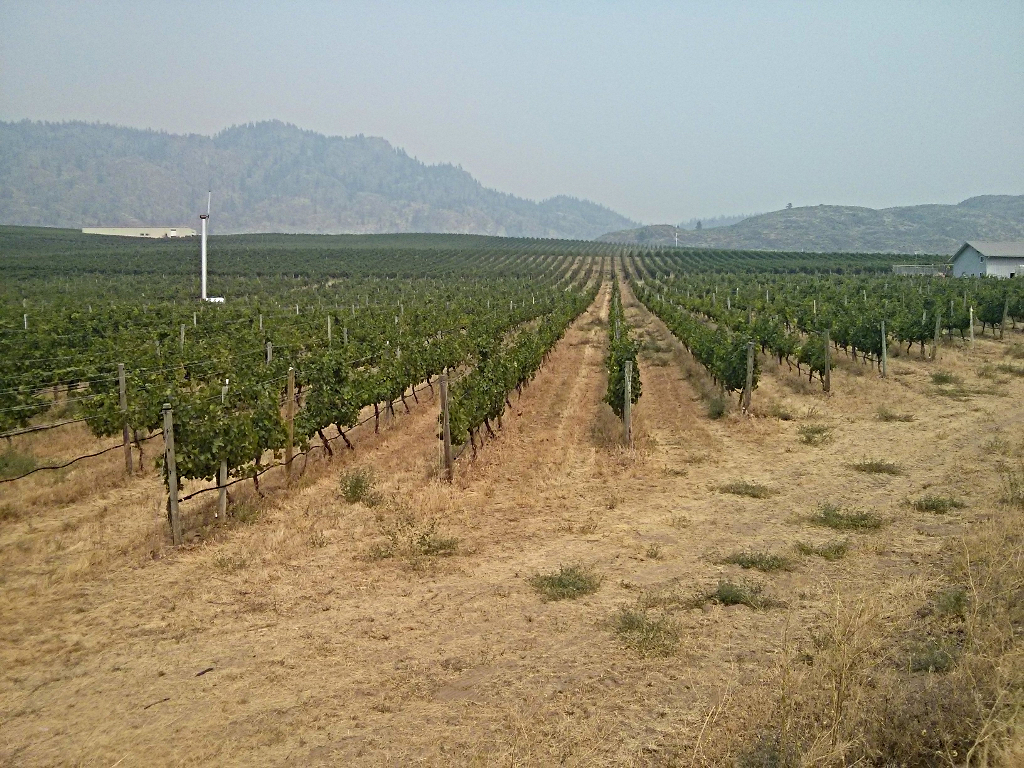
\includegraphics[width=1.0\linewidth]{tmp/photo_culmina_rows.pdf} 
\caption{Typical spacing of vinyard rows. Culmina Winery, Penticton, BC. August 2017.}
\label{fig:photo_culmina_rows}
\end{figure}

\begin{figure} %[htbp] % htbp stand for "here", "top", "bottom", "page"
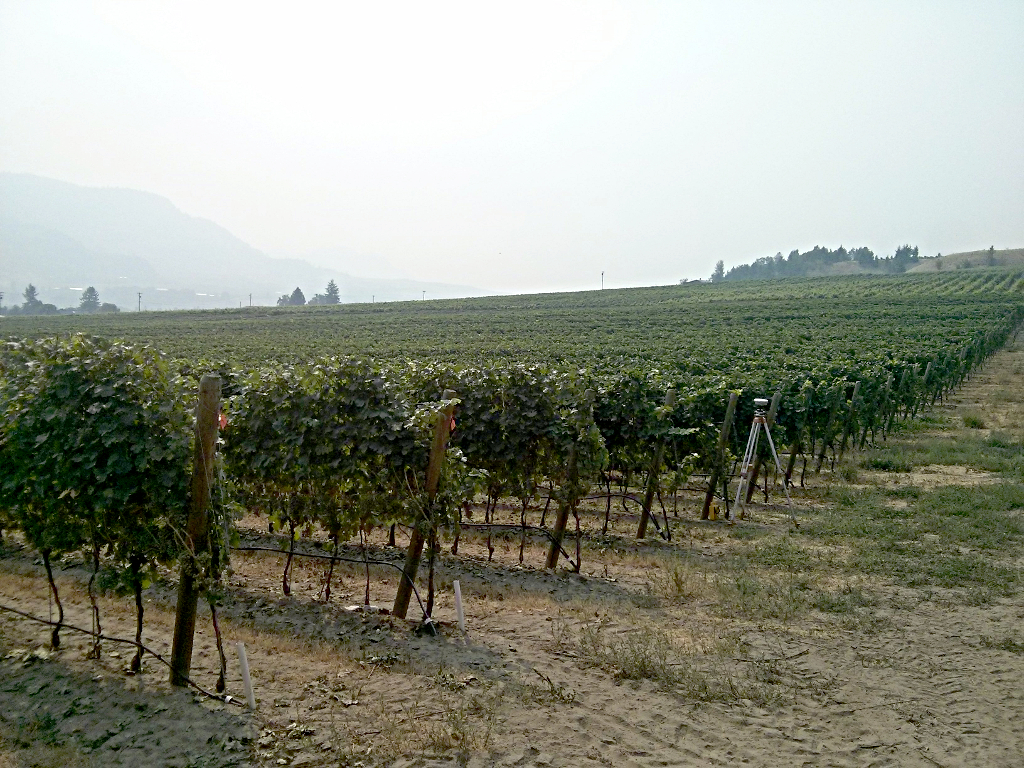
\includegraphics[width=1.0\linewidth]{tmp/photo_culmina_rows_slope.pdf} 
\caption{Low-frequency surface height variation, Culmina Winery, Penticton, BC. August 2017.}
\label{fig:photo_culmina_rows_slope}
\end{figure}


\subsection{Splines}

\begin{figure} %[htbp] % htbp stand for "here", "top", "bottom", "page"
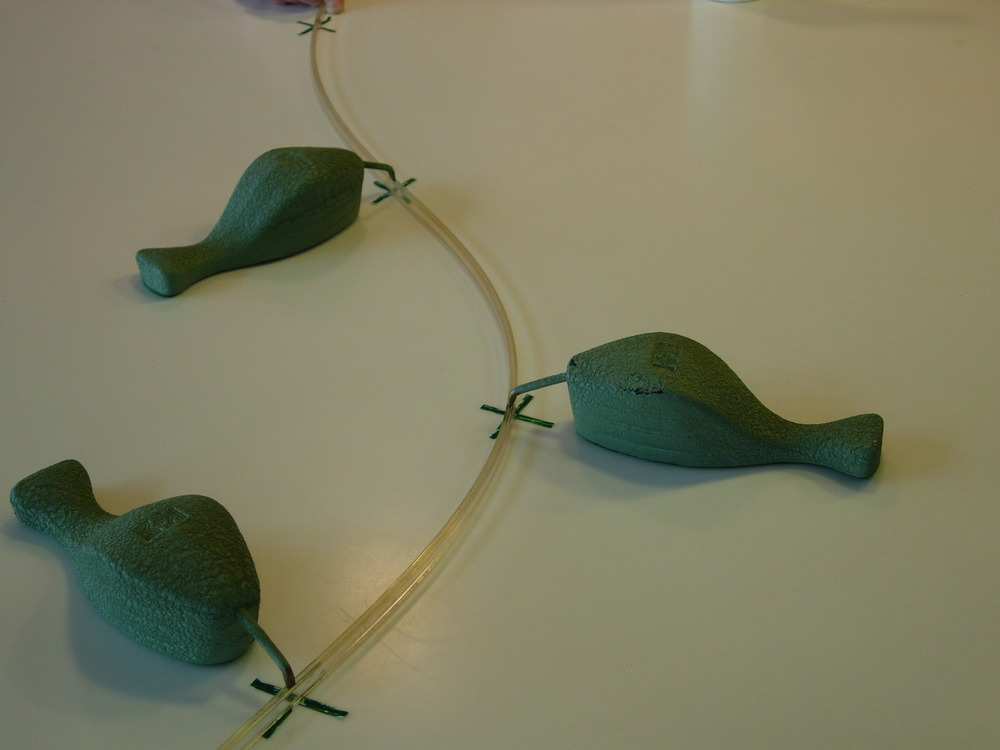
\includegraphics[width=1.0\linewidth]{tmp/draftspline.pdf} 
\caption{A draftsman's spline and ``ducks.'' \parencite{DeBoor2006}}
\label{fig:spline}
\end{figure}

The word ``spline'' originates in drafting, where long, flexible wooden or plastic beams, called splines (figure \ref{fig:spline}), were used to model curves. A spline would be placed on the drawing, held down by two or more lead weights called ``ducks,'' and would seek a shape which minimized the energy stored in the beam. The spline could thus be considered an optimal interpolator \parencite{Wegman2016}. 

In mathematics, the spline is consists of a set of piecewise (usually cubic) polynomials, one each between each pair of ducks, or ``knots.'' At each knot, the first, and possibly higher, derivatives of the adjoining polynomials are held equal, resulting an a curve that is smooth and differentiable along its entire length. The minimum-energy constraint is modelled by minimizing mean square curvature of the polynomial \parencite{Wegman2016}.

In this instance, the spline function is used to model the behaviour of a physical body in space, with velocity and acceleration given by the first and second derivatives, respectively. The second derivative is of particular interest because it is constrained by the aircraft's dynamic properties given by Newton's second law,

\begin{equation}
F = ma,
\end{equation} 

where $F$ is force, in Newtons, $m$ is the mass of the vehicle in kg, and $a$ is the acceleration in $m/s$. Forces on the airframe are generated by the propulsion system, gravity and aerodynamic drag. When the second derivative is positive, its magnitude can be no greater than the acceleration provided by the net of these forces (climbing under maximum thrust). When negative, its magnitude can be no greater than net of these forces with thrust set to near zero (freefall). These constraints may be derived from the aircraft's thrust, as documented by the manufacturer, and its mass and air resistance, which must be measured. 

Though cubic splines are smooth and twice differentiable, it will be observed that the second derivative (acceleration) is not smooth, having cusps at the knots (figure \ref{fig:cubic_derivatives}.) For any polynomial, for some value of $m > 0$, the $m$th derivative will be linear; for cubic splines, this occurs at $m = 2$. This is not a concern, so long as the change of thrust by the aircraft's flight controller is assumed to occur instantaneously. It does not, of course, as it takes time to supply the motors with power, and for their rotational velocity to change. Here, the maximum thrust, or some multiple less than $1$ will be used as an estimate of the limit.

The mechanical spline and its mathematical equivalent are interpolators and pass through each of the knots. A variation on the interpolating spline, the weighted spline, allows the calculation of a weight, applied at each knot, which can suppress the tendency for overshoots \parencite{lancaster1986curve}. However this breaks the continuity of the second derivative, which in turn breaks the physical model.


\subsection{Smoothing Splines}

An alternative construction -- the smoothing or approximating spline -- allows the spline preserve the overall shape of the data distribution without passing through each knot exactly

A smoothing spline has two conflicting objectives \cite{lancaster1986curve, Drakos2002, Boor2001, Reinsch1967}:
\begin{enumerate}
\item To minimize the sum of squared distances between the function estimate and the ordinates;
\item To minimize the curvature of the function.
\end{enumerate}

This leads to de Boor's formulation,

\begin{equation}
S(x) = p \sum_{i=1}^{n} \left( {(Y_i - \hat{f}(x_i))^2 \over {\sigma_i}^2} \right) + (1 - p) \int{ \left( \hat{f}^{(m)}(x) \right)^2 } dx,
\end{equation}

where the first operand is essentialy a Chi-square measure of the function and the second a measure of its curvature, both weighted by $p \in{[0-1]}$ or its negation. Here, $Y$ is the ordinate, $\hat{f}$ is the spline estimate and $\sigma$ represents the variance of the data. $p$ has the effect of controlling the number of knots: as $p$ approaches $1$, the first term is emphasised, forcing a closer fit to the data, while as $p$ approaces $0$, the integral is emphasized, forcing a straighter (smoother) curve. 

The system is constrained, such that,

\begin{equation}
S(x_{i-1}) = S(x_i),
S'(x_{i-1}) = S'(x_i), and 
S''(x_{i-1}) = S''(x_i).
\end{equation}

That is, at each knot, the ends of adjoining splines have not only the same value, but the same first (slope) and second (curvature) derivatives. (In this usage, the function value is the vehicle altitude with the first and second derivatives representing velocity and acceleration, respectively.) To find the spline function, it is possible by indefinite integration to find the original function, beginning with the slopes at the end of the segment and two knots. In the case of the so-called ``natural spline'', the second derivatives at the first and last knots are held to zero. 

Figure \ref{fig:cubic_derivatives} shows a preliminary study of the cubic smoothing spline and derivatives computed on a real-world LiDAR point cloud, using the concave hull ($\alpha = 10m$) for surface-point extraction.

\begin{figure} %[htbp] % htbp stand for "here", "top", "bottom", "page"
\includegraphics[width=1.0\linewidth]{tmp/splines_derivs_smooth_0_5_weight_0_1.pdf} 
\caption{Smoothing cubic spline through the vertices of concave hull derived from a real-world point cloud. First and second derivatives correspond velocity and acceleration, assuming horizontal velocity of 1m/s.}
\label{fig:cubic_derivatives}
\end{figure}

It is evident that the smoothing spline is a good candidate for examination as a trajectory function, as its derivatives provide a means of modeling the physical dynamics of the vehicle and it can be adjusted to satisfy the dynamic and data-quality constraints. The ability to interpret the general shape of a surface without interpolating all points exactly -- which would result in deleterious, difficult-to-resolve artifacts -- is a boon.

What remains is to develop a methodology for selecting weight and smoothness parameters appropriate to these constraints, given the available instrumentation and computational resources.


\section{Methods}

The input to the process described in this study is a sorted (in the y-dimension) two-dimensional (planar) point cloud, oriented in the y-z axis of the aircaft, that is, vertical and fore-aft. The output is a set of parameterized splines that the vehicle will use to set its altitude as it flies.

There is an difficulty with the UAV use-case: the point cloud isn't complete at any time during the flight, so the trajectory must be computed piece-wise in real-time as sufficient data is obtained. Once a trajectory is computed it must not be altered by newly-arrived data, lest discontinuities appear in the trajectory (as its vertical position might jump at any given position between times $t$ and $t+1$.) One way to overcome this difficulty might be to compute the spline over ``blocks'' of point cloud: when a block is assumed to be complete, it is considered ``finalized'' and the trajectory extracted from it. If the spline is computed with the ``natural'' constraint ($S''(x_0) = S''(n) = 0$) then the vehicle's throttle setting can be assumed to remain constant accross each block boundary. It remains to determine whether enough points can be collected, finalized and processed for each block in time to provide useful trajectory information to the vehicle before it crosses the next boundary.

As this issue remains unresolved, this paper focuses on the development and analysis of a spline that covers the entire, intact point cloud.


\subsection{Surface Reconstruction}

Some representation of the imaged ``surface'' must be extracted from the point cloud. If this were not done, points from the interior of the vegetative canopy or the terrain would weight the spline, dragging it downward, degrading the data and possibly precipitating a crash. The point subset must contain enough points to provide some surface detail and few enough to maintain computability. 

However, the definition of a ``surface'' is problematic -- the points represent measurements of real objects, but tell us nothing about what exists between those objects. One possible conception of the surface would be that our certainty about the height of the surface is absolute at the location of a point, A, and degrades with distance from that point. As this distance increases, though, the distance to a neighbouring point, B, decreases, and our certainty about the height of the surface as given by B increases. This implies a kind of probabilistic, interpolating surface implied by the measurements. In the discussion below, the interpolation turns out to be linear.

A simple, fast way of extracting a surface from a 2-dimensional point cloud is to extract the convex hull. Unfortunately, on surfaces that have anything other than a convex, or domed, shape, all of the surface detail would be lost. A better solution would be a concave hull, which would allow for indents in the surface. Unlike the convex hull -- the unique minimum polygon containing the point-set -- there is no single definition of a concave hull. Alpha shapes \cite{Edelsbrunner1994} are a well-defined candidate, but require the triangulation (via Delaunay) of the entire pointset. Another alternative is to modify an existing fast convex hull algorithm to limit the maximum segment length.

The Mototone Chain convex hull algorithm (\cite{Andrew1979}) runs in linear time on a sorted pointset, which is the expected state of the input. By modifying the main loop of the algorithm to limit the length of any given segment, and running it only on the upper surface of the input, it becomes a configurable surface-extraction tool. However, though the maximum segment length can be enforced, there can be no minimum. This leads to possible clustering of vertices near highly curved sections of the surface.

With the convex hull computed on the input point cloud, its vertices can be extracted to form the surface point-set.

\subsection{Spline Extraction}




\section{Proposal}

To show that the smoothing spline is an appropriate mechanism for computing trajectories for remote-sensing UAVs, it will be necessary implement a computational pipeline to determine the spline coefficients from a stream of measurements. The steps in this pipeline entail, in part,

\begin{enumerate}
\item calculating each 2-dimensional Cartesian coordinate based on the measured range, the position and  orientation of the UAV's body frame relative to the intertial frame, and the position and orientation of the laser relative to the body frame;
\item filtering the point cloud to only include relevant points (e.g., by excluding points to the rear of the vehicle);
\item implementing an online concave hull algorithm with the segment-length modification;
\item configuring and computing the spline using the vertices of the concave hull.
\end{enumerate}

These steps will be performed using existing LiDAR point cloud extracts produced by the Hyperspectral-LiDAR Research Group at the University of Victoria, using a DJI Matrice 600 hexacopter and a Velodyne VLP-16 LiDAR. The point cloud will be modified to mimic the output of the scanning laser rangefinder by extracting a swath from the point cloud, measuring the Cartesian distance from an origin to each point (the y-coordinate) and keeping the z-coordinate.

It will then be necessary to quantify the suitability of the spline coefficients by calculating, for example,

\begin{enumerate}
\item the error between the altitude of the trajectory and the elevation of actual terrain (as modeled using standard GIS techniques), at a suitable interval;
\item the error between the altitude of the vehicle and the the trajectory at any point, given its dynamic properties, including whether the vehicle can navigate a trajectory at all.
\end{enumerate}

The first error is important, as the altitude error is a proxy for the variability of data quality. The second determines whether or not the vehicle will crash, but also gives some sense of how much power it must use, and whether it must exceed its nominal capabilities.

The deliverables from this effort will include,

\begin{enumerate}
\item a command-line program to execute the simulation pipeline in approximately real-time using an excisting point cloud and;
\item scripts required for calculating the above errors and any other relevant metrics that come to light;
\item a final report.
\end{enumerate}

Hopefully, products of this activity will provide the first steps towards a field-configurable surface-following UAV flight control system.

\newpage

\printbibliography

\end{document}